\changepapersize{305.3mm:210mm}
\customtag{largepage}

{
	\LARGE
	\noindent Frequency of Releases\par
	\vspace{0.2cm}
}

\begin{multicols}{3}
	\noindent
	\begin{minipage}{\columnwidth + \columnsep}
		\begin{tabular}{|r|l|}
			\hline
			Descriptive statistics & Time between releases \\
			\hline
			count                  & 60                    \\
			mean                   & 20 days 15:11         \\
			std                    & 47 days 00:10         \\
			min                    & 0 days 00:00          \\
			25\%                   & 1 days 00:00          \\
			50\%                   & 3 days 00:00          \\
			75\%                   & 26 days 18:00         \\
			max                    & 338 days 00:00        \\
			\hline
		\end{tabular}
		\captionof{table}{Release statistics}
		\label{tab:release-statistics}
	\end{minipage}
	\columnbreak
	\noindent
	\begin{minipage}{\columnwidth}
		\frame{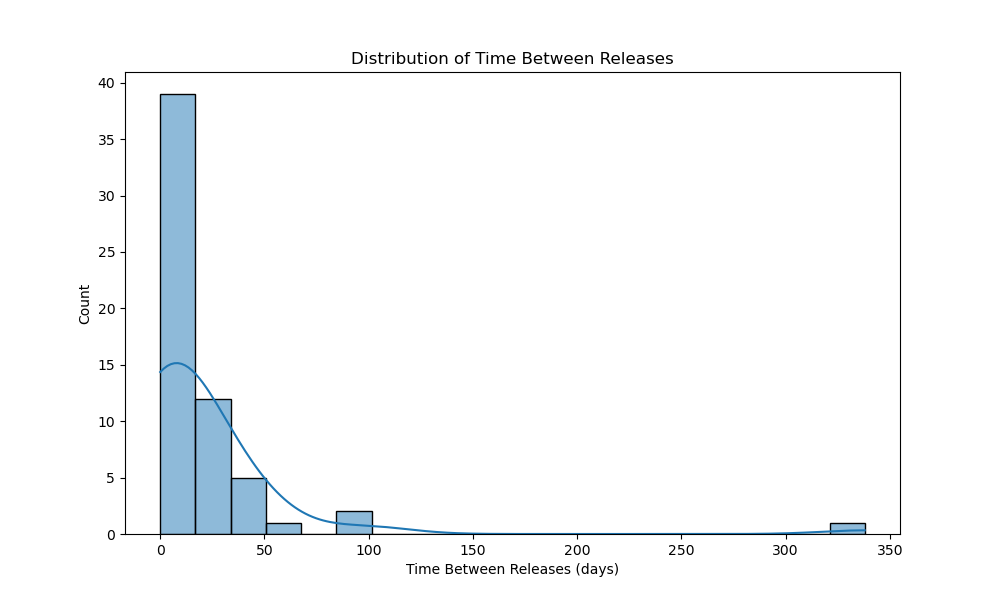
\includegraphics[width=\linewidth]{images/time_between_releases_histogram.png}}
		% \includegraphics[width=\linewidth]{graph2}
		\captionof{figure}{Graph that spans one column}
		\label{fig:releases-histogram}
	\end{minipage}
\end{multicols}

\begin{figure}[h!]
	\centering
	\frame{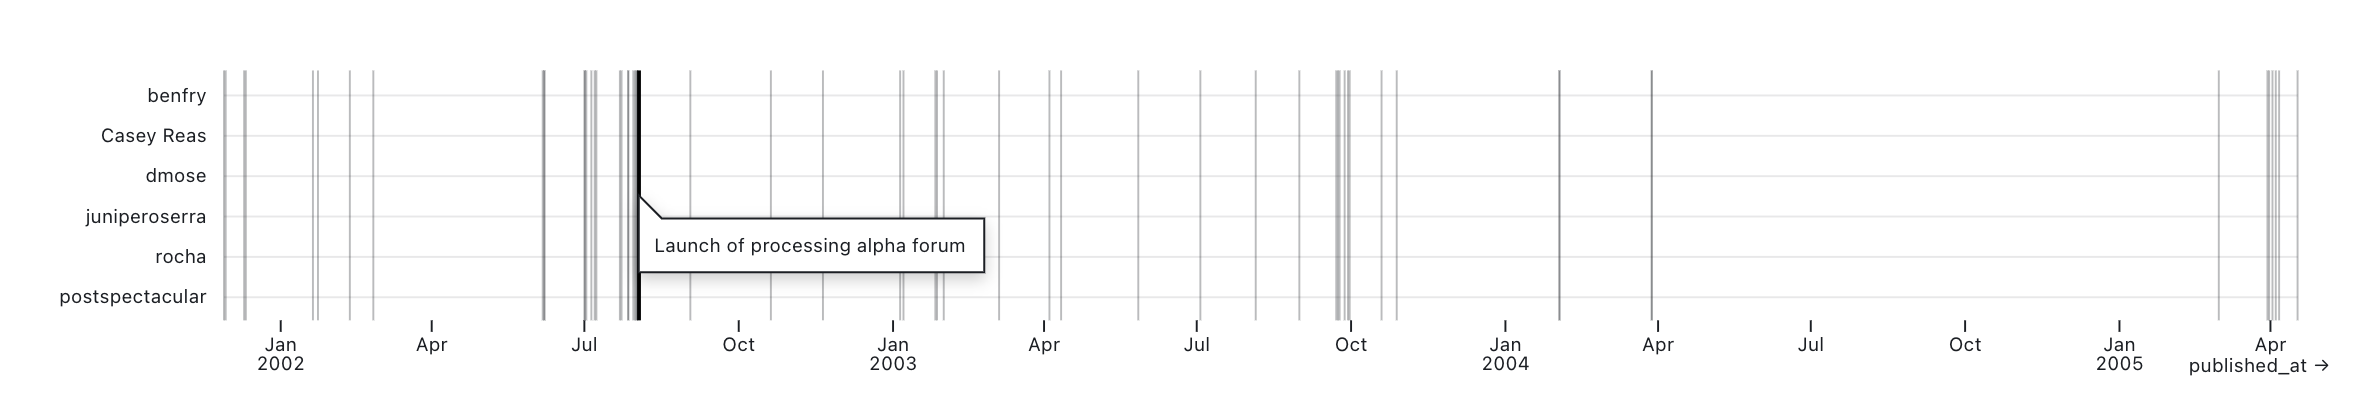
\includegraphics[width=1\textwidth]{images/releases-lines.png}}
	\caption{Time between releases}
	\label{fig:releases-lines}
\end{figure}

% \begin{figure}[h!] 
%   \centering
%   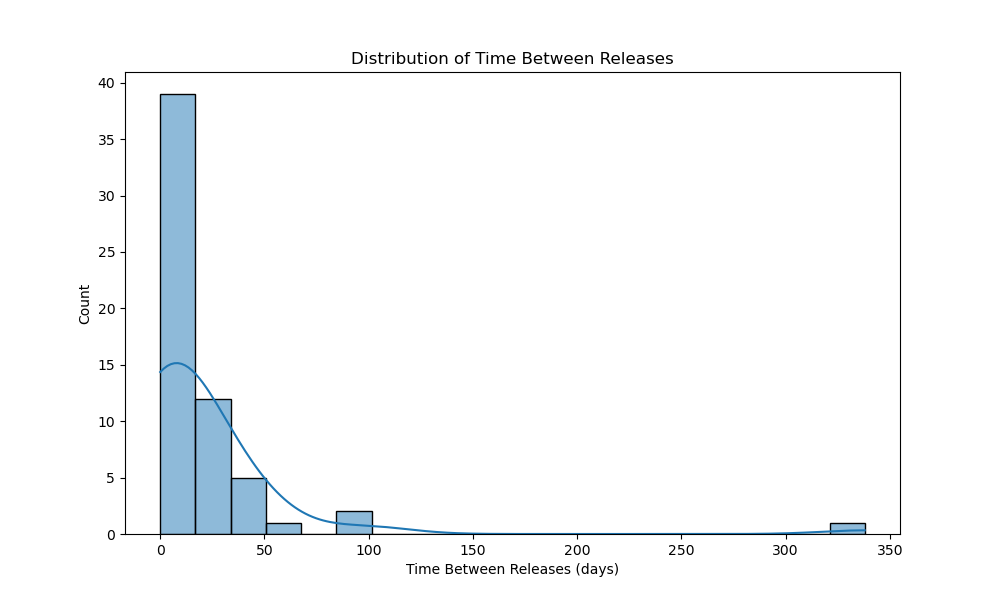
\includegraphics[width=0.9\textwidth]{images/time_between_releases_histogram.png} 
%   \caption{Time between releases histogram}
%   \label{fig:releases_frequency_histogram}
% \end{figure}

\begin{multicols}{3}
	\noindent
	The graphical representations depict a distinctive pattern of release clustering, a testament to the sporadic and intermittent nature of the project's development lifecycle. A notable surge can be observed leading up to pivotal milestones, such as the alpha forum's initial release, indicating a focused burst of activity during these critical junctures.
	\noindent
	The distribution of releases further accentuates the project's non-linear progress, with a marked increase in releases as key points approach, followed by periods of relative inactivity. This ebb and flow suggest that the development process is influenced by external factors or revolves around specific events, leading to a "feast or famine" scenario in terms of updates and improvements.
	\noindent
	Moreover, the extended intervals devoid of any releases could imply that the project advancement is perhaps a secondary or parallel endeavor for the contributors.
\end{multicols}

\defaultareasettings

